\subsection{Model description}
\label{sec:bestlds:theory:model}

Let $y_t$ denote the $q$-dimensional observation at time $t$. Concretely, we assume that $y_t$ is emitted as Bernoulli noise from a latent dynamical system with $p$-dimensional linear-Gaussian dynamics, potentially driven at each time-step by an $m$-dimensional input $u_t$. That is:
\begin{align}
\begin{split}
    x_0 &\sim \mathcal{N}(\mu_0, Q_0) \\
    x_t \mid x_{t-1} &\sim \mathcal{N}(Ax_{t-1} + Bu_t, Q) \\
    z_t &= Cx_t + Du_t \\
    y_t \mid z_t &\sim \textrm{Bernoulli}(f(z_t))
\label{generative_model}
\end{split}
\end{align}
\noindent where $\mu_0, Q_0$ parameterize the initial distribution for the latent variable, $A$ and $B$ refer to the autoregressive and input-driven components of the mean of the latent dynamics, and $Q$ is the covariance of the latent Gaussian noise. The quantity $z_t$ is a latent convenience variable describing the state of the LDS in the $q$-dimensional output space as a linear transformation of the latent state by the output matrix $C$ and the input-output interactions matrix $D$. Finally, the outputs are sampled from a Bernoulli distribution with mean $f(z_t)$ for an arbitrary function $f$ (generally taken to be either the logistic or probit function). (Figure~\ref{fig:bestlds:1} shows a model schematic.)
\begin{figure}[t!]
\centering
    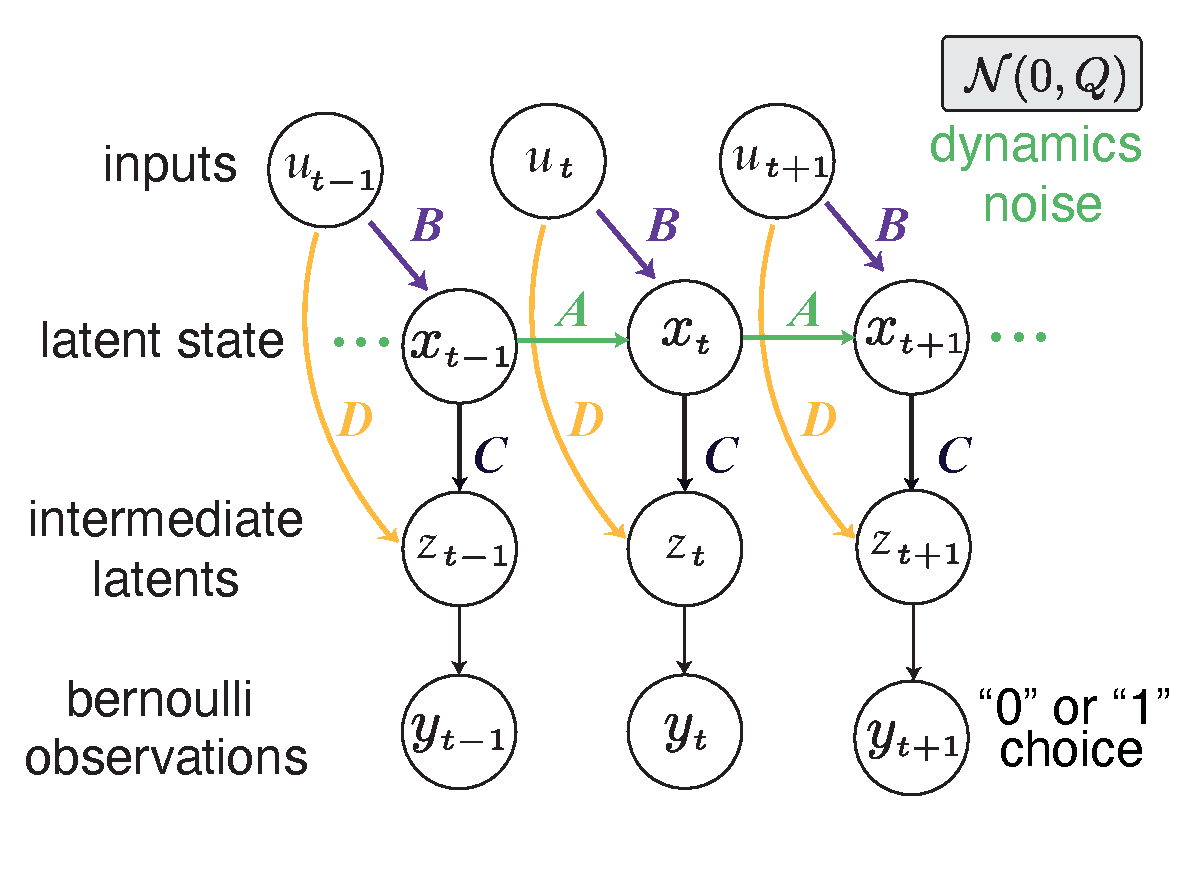
\includegraphics[width=0.65\linewidth]{ch4-bestlds/bestlds-figures/fig1.pdf}
    \caption[Generative model schematic]{\textbf{Generative model schematic.}}
    \label{fig:bestlds:1}
  %\vspace{-1.0cm}
\end{figure}